
%%
%% This is file `example/bare_thesis.tex',
%% generated with the docstrip utility.
%%
%% The original source files were:
%%
%% install/buptgraduatethesis.dtx  (with options: `bare-thesis')
%% 
%% This file is a part of the example of BUPTGraduateThesis.
%% 

\documentclass[%
  degree=master,%
  classlevel=open,%
  mathfont=mathptmx,%
  dedication=false,%
  chapbib=false,%
  finish=print,%
  driver=xetex]{buptgraduatethesis}

%% 自定义导言区
%% 在这里添加你需要的宏包、自定义命令、环境等
%% \usepackage{...}
%% \DeclareMathOperator{\CT}{H}
%% \DeclareMathOperator{\Cov}{Cov}
\def\BUPTThesis{\textsc{BUPT}\-\textsc{Thesis}}

%% 在这里添加图片文件搜索目录
\usepackage{graphicx} 
\usepackage{algorithm}  
\usepackage{algorithmic} 
\graphicspath{{../}{image/}{image/highres}}
%% 自定义导言区结束

%% 加载缩略语定义
%%
%% This is file `example/metadata.tex',
%% generated with the docstrip utility.
%%
%% The original source files were:
%%
%% install/buptgraduatethesis.dtx  (with options: `metadata')
%% 
%% This file is a part of the example of BUPTGraduateThesis.
%% 

%% 涉密论文保密年限
\classdur{三年}

%% 学号
\studentid{2011000000}

%% 论文题目
\ctitle{北京邮电大学研究生学位论文\LaTeXe{}模板使用示例文档}
\etitle{Example of BUPT Graduate Thesis \LaTeXe{} Template}

%% 申请学位
\cdegree{工学硕士}

%% 院系名称
\cdepartment{信息与通信工程学院}

%% 专业名称
\cmajor{移动通信}

%% 你的姓名
\cauthor{学生姓名}

%% 博士后研究工作报告-分类号
\classnumber{O441.3}

%% 博士后研究工作报告-UDC
\udc{621.396.9}

%% 博士后研究工作报告-学校编号
\schoolserial{147227}

%% 博士后研究工作起始时间
\startdate{2014年10月29日}

%% 博士后研究工作期满时间
\finishdate{2016年4月2日}

%% 你导师的姓名
\csupervisor{导师姓名}

%% 日期自动生成,也可以取消注释下面一行,自行指定日期
\cdate{\CJKdigits{2013}年\CJKnumber{12}月\CJKnumber{25}日}

%% 中文摘要
\cabstract{%
  中、英文摘要位于声明的次页,摘要应简明表达学位论文的内容要点,体现研究工作的核心思想。
  重点说明本项科研的目的和意义、研究方法、研究成果、结论,注意突出具有创新性的成果和新见解的部分。

  关键词是为文献标引工作而从论文中选取出来的、用以表示全文主题内容信息的术语。
  关键词排列在摘要内容的左下方,具体关键词之间以均匀间隔分开排列,无需其它符号。
}

%% 中文关键词,关键词之间用 \kwsep 分割
\ckeywords{\TeX \kwsep \LaTeX \kwsep xeCJK \kwsep 模板 \kwsep 排版 \kwsep 论文}

%% 英文摘要
\eabstract{%
  The Chinese and English abstract should appear after the declaration page.
  The abstract should present the core of the research work, especially the purpose and importance of the research, the method adopted, the results, and the conclusion.

  Key words are terms selected for documentation indexing, which should present the main contributions of the thesis.
  Key words are aligned at the bottom left side of the abstract content.
  Key words should be seperated by spaces but not any other symbols.
}

%% 英文关键词,也用 \kwsep 分割
\ekeywords{%
  \TeX \kwsep \LaTeX \kwsep xeCJK \kwsep template \kwsep typesetting \kwsep thesis}


\loadglsentries{acronyms}

%% 攻读学位期间发表论文
%% 用 \newcite{<suffix>}{<caption>} 声明不同的论文类型(例如: 期刊论文、会议论文等)。每一个类型的对应的 .bib 文件用 \bibliography<suffix> 命令加载,用 \nocite<suffix> 命令引用。具体请参考 pubs.tex 中的示例
\newcite{jrnl}{期刊论文}
\newcite{conf}{会议论文}
\newcite{patent}{专利}

\begin{document}
%% 声明前置部分
\makefrontmatter

%% 主体部分
\mainmatter
%% 用\include{}命令引用各章.tex文件
\chapter{绪论}
\section{课题研究的背景与意义}
\subsection{研究背景}
自从人类第一次张开眼睛观察世界开始,图像这一最早的原始信息传递媒介就开始以各种各样的形式在人类的信息传递过程中发挥着非彼寻常的作用,正所谓“一图胜千言”,“耳听为虚,眼见为实”说明的正是这个道理。随着图像的表现形式不断的发展和图像数据的日益增加,如何提取图像中所包含的海量信息以及信息的分析使用成了现代多媒体,人工智能,自动化控制等多个领域都亟需解决的问题。近些年来图像领域人工智能迅猛发展,神经网络技术因为简单,高效,对于数据适应性强等特性,在各种图像识别的领域大规模训练使用,取得了非常好的效果。人脸领域受相关技术的影响,有了很大的进步,从慢慢接近人眼的便是效果,到不断超越,以至于后来的百万级人脸搜索百分之99的准确率,可以说正在慢慢朝着实用化的技术发展,成为整个深度学习技术革命的排头兵。
\subsection{研究意义}
在人脸领域之中,包含人脸检测、人脸landmark点、人脸识别、人脸属性识别等多个分支。其中人脸识别是图像信息中具有身份信息生物特征的一部分,可以广泛的用在安防,娱乐,多媒体等领域。而如果说人脸识别是识人,辩人。那么人脸属性识别就可以说是“相面算命”了,比如说人机交互中的表情识别互动,又比如说视频播放网站中限制级视频对于低龄观众限制,尤其在用户数据统计的过程中一张人脸图片,就可以识别出用户性别,年龄,是否戴眼镜,基本面部特征,发型状态等信息,从而可以进行个性化的业务分析与定制推荐,这在逐渐强调个性化发展的社会中具有很高的市场。

但是人脸属性作为一项人脸中的重要研究领域,在深度学习中的技术进展却总是不温不火,无论是准确率还是实际使用都有一定的发展空间。其中主要的问题在于网络结构上对于人脸属性多样性兼容问题,以及人脸属性任务对于人脸图片数据要求的复杂和严格性,人脸属性种类繁多,且人脸场景分布极为复杂,标注工作难度较大,且歧义性较大。因此,本文旨在在深度学习对于图像识别任务有较大推动的今天,研究网络结构和数据分布对于属性识别的影响。从属性识别的网络结构探索和不同数据分布整合对于属性数据的提高效果。同时结合迁移学习的思想为提高不同环境下人脸属性的识别准确率。
\section{国内外研究现状}
\subsection{人脸属性的任务目标发展}
从时间角度来看,基于人脸图像的多种人脸属性预测估计在上世纪90年代就开始,1990年,MIT的Cottrell和Metcalfe把基于AutoEncoder的特征降维用于性别和表情识别\cite{EMPATH};1999年,塞浦路斯学院的Lanitis构建了FGNET年龄估计数据库(共82人,1002张图像),当时用PCA做特征提取\cite{FGNET};2006年,北卡的Ricanek 和 Tesafaye构建了首个大规模年龄、性别、种族数据库MORPH(1.3万人,5.5万图像)\cite{MORPH};2008年,哥伦比亚大学的Kumar等人构建了包含10个属性(后在期刊文章里扩展到60多个)的大规模名人数据库PubFig(共200人,6万张图像)仅部分公开,提取了手工设计特征,之后对每个属性训练SVM\cite{FACETRACER};2010年,MIT的Pho等人首次研究了基于普通摄像头的非接触式心率估计,这是“由表及里”的一次突破;2015年,中科院计算所VIPL研究组首次研究了人与机器在属性识别上的性能差异(可控),并发现机器在年龄、性别和种族的识别上已经可以超过人类\cite{HUHAN};NIST组织了年龄和性别预测方面的评测竞赛,并且出了一个报告概括了领域相关工作\cite{FERET};此外,香港中文大学汤老师组构建了大规模互联网名人的40个属性数据集celeA\cite{CELEA}。由此可见,研究工作的时间跨越度并非很大,但是各方面工作的丰富性和多样性还是令人瞩目的。
\subsection{人脸属性识别方法变化}
从特征的表示方法来看,是一个从全局特征、细节特征到深度特征的过程,具体来讲:全局表观特征:包括Intensity、PCA\cite{PCA}、BIF生物启发式特征\cite{BIF},局部二值模式LBP(Local binary patterns)\cite{LBP},加窗傅立叶变换(Gabor)等。细节特征如:主动外观模型AAM(Active  Appearance  Model)\cite{AAM},
纹理,肤色,人脸形状,sift特征等。深度学习特征\cite{ADIENCE}\cite{CNNSVM}如CNN,DNN中网络的不同层卷积输出。其中是一个不断演变但是也时有结合的过程。从特征分类方法上来看:研究的任务形式也从单任务学习(常用方法:每个属性训练一个分类器)慢慢演变到多标签学习\cite{CELEA}\cite{HUHAN}(回归目标不仅是数,而是向量形式)而后根据不同的细粒度额精确化需求,发展出层级式的分类器(由粗到细,特别适用于年龄分类,如先确定年龄范围,再进行具体年龄分类)和多任务学习\cite{MULTITASK}(多任务限制玻尔兹曼机,多任务CNN等等)。总结来看,是一个从手工设计特征到深度特征、从组合式的学习到端到端学习、从STL到MTL(从单任务学习到多任务学习)的发展过程。

人脸视觉属性学习并不简单,特别是在非可控的真实场景下。影响因素有以下几个方面:传感环境(尤其在室外)的不可控性以及人物的不配合性,这会引起姿态、光照、遮挡等多种因素的影响;属性之间的相关性以及差异性;属性数量的增多引起内存消耗的增加,因此需高效的模型。
\section{本文的工作与贡献}
\subsection{研究内容}
在本文的主要研究的内容有两个,第一项是结合人脸属性的性质探究在人脸属性在深度学习技术下的表现。其中包括人脸属性数据的总结与整理,规划人脸属性的标注类型,单任务模型下的人脸属性的表现,多任务模式下人脸属性的表现等,主要的衡量指标是在不同模型组合和模型策略的情况下人脸属性模型的准确率。另一方面,是针对于现实环境中图片采集的不可控制性,使用对抗生成网络来模拟不同场景的人脸数据,并且探究如何使用迁移学习的思想来对提高人脸属性对于不同场景泛化能力。在这一任务中,除了最终对于人脸属性的准确率提升之外,人脸图片的生成质量也是衡量得指标之一。
\subsection{主要贡献}
在这项研究工作之中主要贡献包括研究内容上的工作和一定的工程优化工作,具体如下:
研究上的工作:
根据人脸属性任务的性质,基于Alexnet\cite{ALEXNET}设计人脸属性的单任务和多任务网络,保证具有一定的可复用性。
设计具有网络输出置信评估的模块,增加网络对于自身的输出的感知能力,从而可以更加精确的把握模型的输出准确性。
研究对抗生成网络的使用,使用对抗生成网络成功通过噪声模拟出数字,物体和人脸图片,且效果较为逼真。
研究对抗生成网络在图像超分辨率领域上的应用,大幅度提升对抗生成网络的图像生成质量。
并基于此项技术,在不直接使用celeA数据的情况下,仅使用lfwA和对应的超分辨率图像进行训练,提高了模型在celeA数据集上的准确率。
证明基于超分辨率率的迁移学习是可行的。
工程上的工作:
研究如何使用多机多卡的训练,并基于机器学习框架的使用完成了对于人脸属性相关任务的训练,提升了训练和算法迭代的速度。
在具体的网络前馈过程之中,使用多线程、指令集等优化方式,提升识别模型输出的速度,包括人脸属性的概率输出和超分辨率的图片生成的速度。
\subsection{论文的组织结构}
第二章:笔者主要介绍涉及人脸属性在深度学习技术种一些基本常识和常见的操作和笔者对相关瓶颈操作的一些优化。具体包括:
在卷积神经网络的基础操作中介绍所谓卷积操作的多种实现和使用方式介绍,激活函数的具体使用,常见的网络参数初始化方法和网络训练相关细节。
在多机多卡的部分介绍,在多卡训练中数据的同步和分发方式,模型参数的更新策略,多机训练中需要注意的一些关键选项配置,以及如何简单的通过机器学习框架完成多机多卡的训练。
在网络前馈的优化部分会介绍一些实用性非常强的快速卷积算法,如im2col+gemm,Winograd等。对于网络中常见操作的如卷积、batchnorm层的合并等。

第三章
笔者主要介绍针对于在人脸属性所进行的一些实验和创新的过程的一些相关工作,
包括对于人脸属性数据的性质分析、人脸常见数据集的介绍、人脸属性识别中常见的识别方法等。
在此基础上总结了三个人脸属性识别所面临的问题:充分利用标签不同的数据库,选择怎样的预处理方式才有助于人脸属性任务的学习,怎样更加精确的把控人脸属性的模型输出。
并在提出问题的基础上进行了解答,通过数据集并行训练的方式改进问题一,使用人脸矫正固定输入格式改进问题二,加入网络自评估模块改进问题三。

第四章
笔者会介绍如何使用对抗生成网络对于不同场景下的人脸进行学习并且根据噪声生成人脸图片。
使用超像素的方式对于人脸图片进行一定程度上的效果增强和场景迁移。
通过结合迁移之后的人脸图像进行学习可以方便的改进人脸属性中由于数据分布不同导致准确率下降情况

第五章
笔者主要对实验过程做一个综合性的概述并且自我评价一下整个实验过程中出现的问题和解决问题的方法。
回顾在解决问题种反应的一些现实层面的现象以及个人对这些现象出现的原因和结果的思考。
当然也包含一点关于未来和未解决工作的思索。

\chapter{卷积神经网络的相关技术介绍}
\section{卷积神经网络的基础操作和训练}
\section{多机多卡策略对于网络训练的提升}
\section{网络前馈速度的优化}




\chapter{人脸多属性属性识别的架构}
\section{人脸属性数据库简介}
\section{人脸属性识别的单任务模型}
基于人脸属性的单任务模型STL(下称单任务模型),顾名思义就是给定一个图像,建立一个模型去对一个属性进行学习。这不仅是人脸属性识别任务中的常见做法,也是整个模式识别领域基础的框架模式,。
在早期,数据集通常只有一种属性的标注,比如之前提到的FG-NET,它包含82个目标的1002张图像,最初只有年龄属性。作为一个分类问题,一些常见的模式识别方法也被应用其中,例如主动外观模型AAM(Active  Appearance  Model),局部二值模式LBP(Local binary patterns),加窗傅立叶变换(Gabor)等,这些常规的做法,总体来讲还是遵循特征提取工程再加上分类器模型的流程,包括特征相关性的筛选,不同模型的融合等等。但是很多时候根据固定模式提取的特征往往不够具有代表性,与识别任务的关联性不够高。于是大家开始着力想寻找一些相关性更高的方法包括,Fu等将流形学习方法引入年龄估计;另外,Guo等提出了生物启发的特征方法,Hu提出了统计信息特征(Dif,Demographic informative feature)的概念;但是时至今日,CNN特征在图像领域的出色表现,让人们对于单任务模型的使用和理解有了非常大的提高,并且总结出了一套非常简练有效的的框架:
以hu的DIF方法作为对比,hu的基本框架概述如下:前端为特征提取阶段,旨在提取对属性有判别力的特征,而不是完全无监督的。后端连接一个层级式的分类器,用于属性学习。
其中有几个主要部分:DIF(Demographic informative features)特征提取,层级式分类器,人机对于单属性预测任务的对比
1)DIF特征
DIF(Demographic informative features)是基于BIF(生物启发式特征)的。比如,我们输入一个人脸部件,先用Gabor滤波器提特征(12个尺度,8个方向),再做一些池化操作,以减小特征图的数目和维度(6个尺度,8个方向),将得到的特征串成一个4280维的长向量,用来做之后的分类等任务。总体上还是一个无监督的特征处理方法。所以之后,又对此工作做了改进,旨在不仅能够抓住图像细节,还能减小冗余性,提高特征与最终识别任务的相关性。
2)层级分类器的建设
因此,我们之后又引入一些特征学习工作。我们希望从之前的特征集中提取一个特征子集,挑选出最相关的特征,比如:
学习一个新的特征子空间(如LDA)
基于Boosting的特征选择
3)人机性能对比
我们还重点研究了人和机器的性能对比,我们做了当时规模最大的数据集来衡量并对比人和机器的性能。数据集包含以下几个方面:
FG-NET,年龄估计
MORPH(2000张图片),年龄、性别、种族估计
PCSO(2000)张图片,年龄、性别、种族估计
我们在这个数据集上进行了大量的实验,得到了许多有趣结论,接下来详细介绍。


这个工作得益于作者的精心调试和改进,
年龄估计结果对比,使用FG-NET和MORPH数据集,实验显示我们的方法取得了当时最好的结果,具有最小误差,且具有非常好的演示和出色的数学模型和理论推导。
如图显示人和机器的性能对比,可以看出机器识别能力的绝对误差要小于人类。当在做年龄估计时,算法估计偏差比较平衡。而人类往往会将年龄估计偏高。这里是误差分析,我们发现,虽然总体上机器性能高于人,但是机器会犯一些偏离实际较大的低级错误,这也是很多学习算法的共同问题。年龄估计,实验表明,算法对真实年龄和人类标注的表观年龄的估计偏差并不大。总体来讲机器的表现可圈可点。

但是需要注意的是在这个过程中,技术细节较为复杂很可能一个步骤做不好就整个系统崩溃,同时因为图片数据库和过多人工干预导致了一定程度上的局部最优解,在真实场景中,难以取得良好的效果,
得益于现代神经网络的出色表现,单属性预测模型的pipeline得到了极大的简化,同时结合端到端的思想和数据的提升效果,可以很好的提升单属性模型的预测效果。

CNN算法下的单模型输出预测:


我们也做了一些相关性的相关性实验,发现整个模型的效果和时间都较之前有了很大的提升。




\section{人脸属性识别的多任务模型}
近来,很多人脸数据集都有多属性标注。比如,MORPH有年龄、性别、种族三个标注属性。香港中文大学的CelebA数据集含有40个二值属性,如头发、眉毛、鼻子、胡须、性别等。如果针对每一个属性都设计一个模型,那么其模型复杂度过大。因此,能否设计一个模型来实现多属性的识别呢?答案是肯定的,也是可行的。
方法一:标签编码

将多属性标签组合进行编码(比如,将一岁亚洲男性标记为001,将一岁非洲男性标记为002等),将多属性问题转化为分类编码问题,也就是单一属性。
局限性:
但是,对于属性数目较多的情况,这种方式会引起数据的组合爆炸。因此,该方法只适合属性数目很小的情形。
方法二:多标签回归

通过回归的方法,使预测的特征向量与Groud-truth属性向量的损失越来越小,二者趋向接近,由此得到预测的特征向量。
局限性:
在提特征阶段,虽然有几十个属性,但用的都是同样的特征,未考虑不同属性的相关性和差异性。

基于多任务的属性学习

我们更倾向于用的是多任务方式。利用属性之间的相关性,包括正相关和负相关;以及应对属性之间的异质性,比如年龄是可量化的,而种族是类别化的,这就需要不同的处理方式。



\section{人脸属性识别中的网络能力自评估模块的设计}


\chapter{对抗生成网络在人脸属性中的应用}
\section{对抗生成网络相关技术的介绍}
早在2014年,人们对于神经网络技术的研究非常狂热的同时,也有一部分理智的科学家认为神经网络的输出判断具有非常高的风险,输出具有非常高的不稳定性,所谓数据集上的准确率超越人类不过是一场谎言,为了戳穿这一谎言,他们在神经网络判断正确的图片上简单加了一些噪声,对于人类来说根本没有察觉图像的变化,但是在神经网络却完全将其判断成另外一种物体。同时科学家们宣称这样极具欺骗性的图片并非偶然得到,而是可以量产的,比如通过对抗生成网络。

借助于博弈论中的零和博弈思想(在零和博弈中,游戏玩家之间的利益总和是固定的,即一方获得收益,另一方就要承担损失。)Goodfellow极具想象力的提出了可以通过搭建两个对抗的网络,各自的目的就是降低对方的准确率,或者说提升对方loss。通过这样非常具有竞争性的训练过程,最够提升两个网络的性能。具体来讲:在对抗生成网络中,玩家的角色会分别有生成模型(generative model)和判别式模型(discriminative model)充当.生成模型G捕捉样本数据的分布,判别模型D是一个二分类器,估计一个样本来自于训练数据(而非生成数据)的概率。G和D可以是线性代数的算法操作组合,也可以是神经网络的网络模型,都可以理解成或者定义成非线性函数。通过不断调整G和D,直到D不能把事件区分出来为止。在调整过程中,一方面需要优化G,使得它尽可能的让D混淆;另一方面需要优化D,使得它尽可能的能区分出假冒的东西;当D无法区分出事件的来源的时候,可以认为,G和M是一样的。从而,就获得了能够以假乱真的数据。

但是对抗生成网络很明显并不能像正常的CNN网络一样对于具体的模式识别任务,但是作为探究CNN生成原理的一部分,对抗生成网络主要是希望能够了解CNN能够从图像中学习到什么样的信息,怎样学习的,并且能否以较为直观的形式也就是生成图像来表示出来,(尽管学习到的东西很多时候并不能够以图像的形式进行展现)。
\section{探究对抗神经网络的应用}
在之前对于对抗生成网络的介绍中,可以发现对抗生成网络最初是来证明神经网络算法对于数据分布具有一定的局限性。而慢慢发展,人们并不在乎神经网络是否对于数据分布有一定的的局限性,而狂热的希望能够通过对抗生成网络获得以假乱真的机器生成图片。似乎人们觉得如果机器能创造他,那机器肯定可以了解他,那么识别他也是轻而易举。于是乎这种炫酷,但是有一定投机取巧性质的思路不仅开始影响最初使用对抗生成网络探究神经网络有效性的本意,也影响着各种识别任务的传统数据+模型的预测方式。

在现有基于模型和分类算法的场景下,对抗神经网络还很难展现出对于属性任务有明显的提升,而对抗生成网络往往以生成各种图片来获得关注和人们的注意,而在业内确实有一些方法可以生成带有人脸属性的人脸图片。那么是否可以通过生成图片的方式为神经网络增加训练的数据,从而起到为属性识别增添数据的作用就成了对抗生成网络在人脸属性上的应用方向。首先可以从使用对抗生成网络直接生成训练数据的方向入手。
\subsection{使用对抗生成网络生成真实图像}
首先参考了DCGAN\cite{DCGAN}的方法和思路,采用了如下的网络结构作为生成图像的基本架构, 生成模型:输入100维的噪声到第一个全连接层,将其映射为1024维,然后再把1024的一维向量重塑成1024个通道的4x4的特征图。基本规律是生成网络的每一个下一层是反卷积层,通道数减半,图像尺寸加倍。

判别模型:就是一个没有池化层的全卷积网络,输入是生成模型输出的图像,输出一个标量,表示输入数据属于训练数据而非生成样本的概率。
\begin{figure}[h]
  \centering
  \subfigure{
  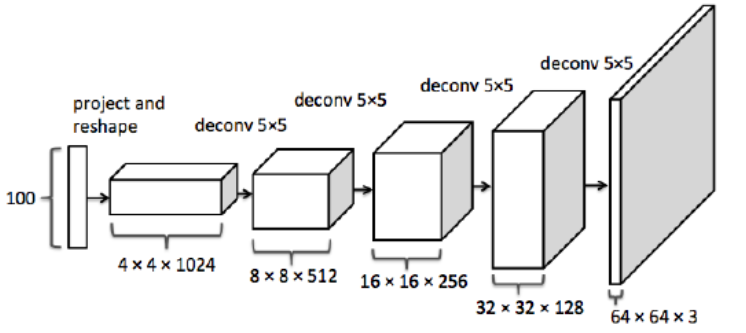
\includegraphics[width=3.0in]{DCGAN_g.png}
  }
  subfigure{
  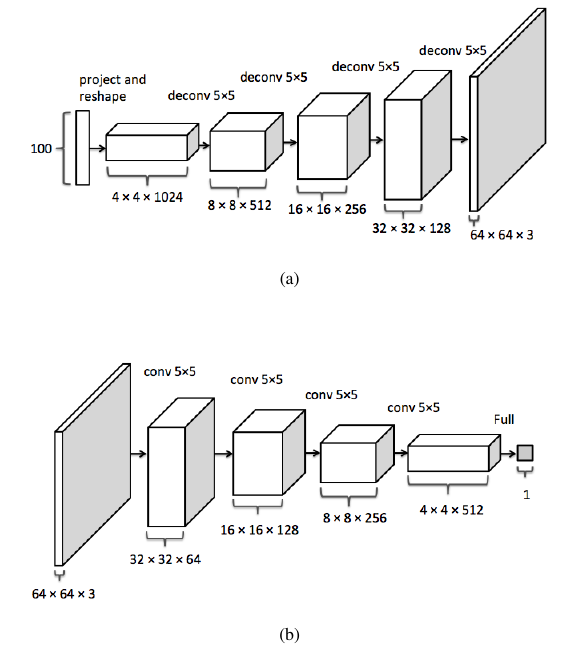
\includegraphics[width=3.0in]{DCGAN_d.png}
  }
  \caption{DCGAN的网络结构:(a)DCGAN中的生成网络模型结构;(b)DCGAN中的判决模型网络结构}
\end{figure}

\subsubsection{生成数字图像}
首先使用mnist数据\cite{MNIST}作为训练样本,实现了从100维的噪声生成数字图像,发现对抗生成网络确实可以生成较为逼真的数字图片,而且生成的图片并不局限于一种状态。
\begin{figure}[!ht]
 \centering 
	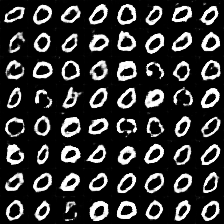
\includegraphics[width=1.0in,height=1.0in]{minnum0.png}
	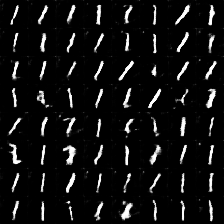
\includegraphics[width=1.0in,height=1.0in]{minnum1.png}
	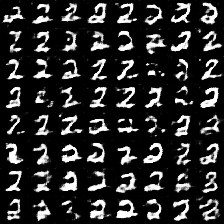
\includegraphics[width=1.0in,height=1.0in]{minnum2.png}
	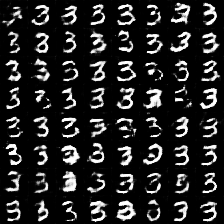
\includegraphics[width=1.0in,height=1.0in]{minnum3.png}
	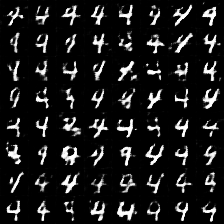
\includegraphics[width=1.0in,height=1.0in]{minnum4.png}
	
\includegraphics[width=1.0in,height=1.0in]{minnum5.png}
	
\includegraphics[width=1.0in,height=1.0in]{minnum6.png}
	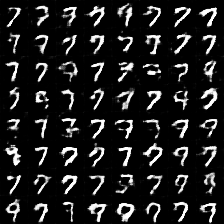
\includegraphics[width=1.0in,height=1.0in]{minnum7.png}
	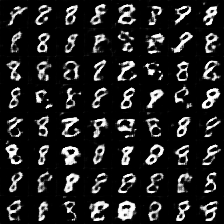
\includegraphics[width=1.0in,height=1.0in]{minnum8.png}
	\caption{minist图片生成的数字图片}
\end{figure}

\subsubsection{生成物体图像}
于是,我们加大了训练的难度,更换cifar10\cite{CIFAR10}数据作为训练的样本,实现了32*32的彩色物体图像生成,但是发现效果似乎并不够出色,在生成的的过程中,虽然能够看物体的生成具有一定的个形状信息和物体轮廓,但是整体的效果却不是很好,不能够生成出具体的能够和真是图像匹配的物体图片。
\begin{figure}[!ht]
 \centering 
	\subfigure[真实的cifar10图像数据]{
	\includegraphics[width=2.0in,height=2.0in]{realGAN.png}
	}
	\subfigure[伪造的cifar10图像数据]{
	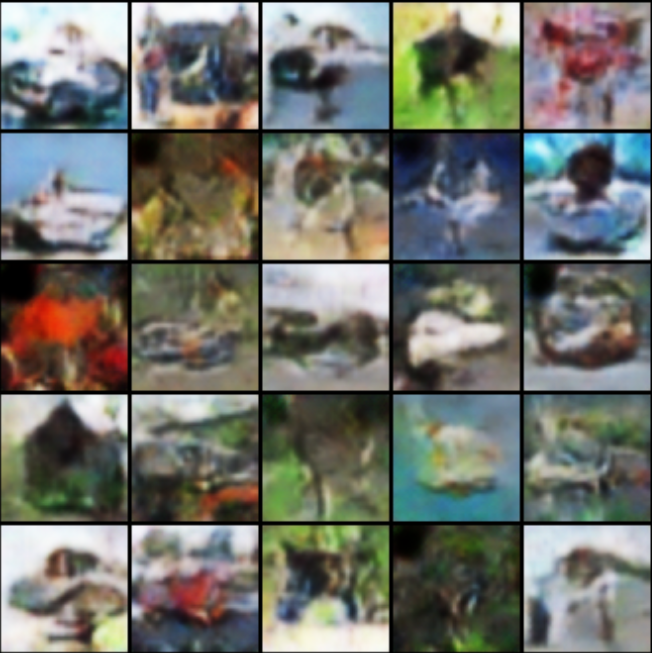
\includegraphics[width=2.0in,height=2.0in]{fake.png}
	}
	\caption{cifar10图片生成的数字图片}
\end{figure}

\subsubsection{生成人脸图像}
那么任务换到在人脸图片的生成上,我们决定放弃DCGAN的结构,装用BGAN\cite{BGAN}和WGAN距离\cite{WGAN}的方式进行人脸图像的生成,事实证明相比于DCGAN,这种方式可以取得更加鲁棒和逼真的效果。

WGAN:

\begin{figure}
  \centering
    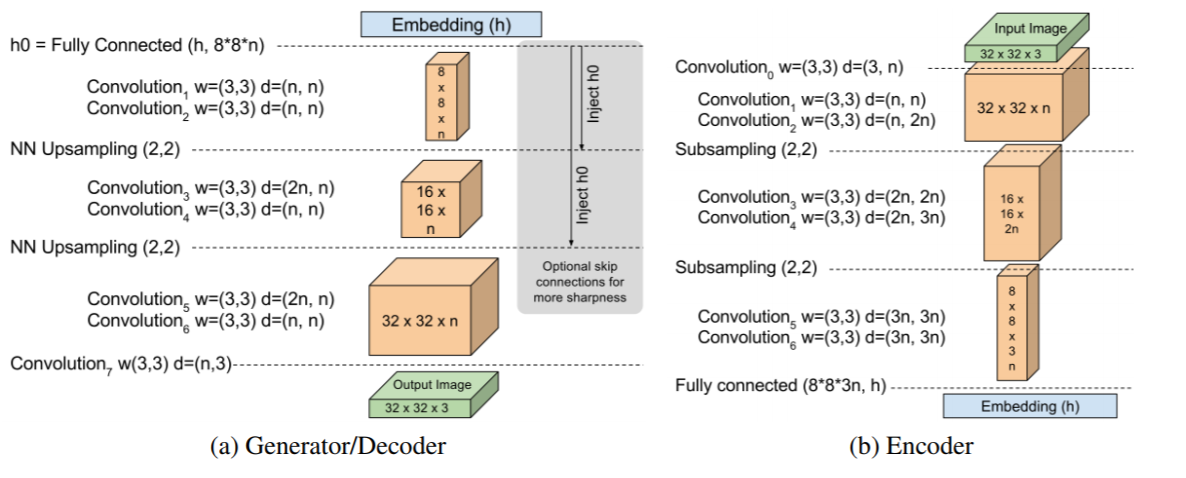
\includegraphics[width=4.0in]{BGAN_struct.png}
  \caption{BGAN的网络结构}
\end{figure}

\begin{figure}[!ht]
 \centering 
	\subfigure[1epoch]{
	\includegraphics[width=1.3in,height=1.3in]{BGAN1.png}
	}
	\subfigure[5epoch]{
	\includegraphics[width=1.3in,height=1.3in]{BGAN2.png}
	}
	\subfigure[10epoch]{
	\includegraphics[width=1.3in,height=1.3in]{BGAN3.png}
	}
	\subfigure[100epoch]{
	\includegraphics[width=1.3in,height=1.3in]{BGAN4.png}
	}
	\caption{人脸图片生成效果图}
\end{figure}
结果显示在人脸生成的过程之中,可以产生非常具有迷惑性和真实性的人脸,是对抗生成网络作为人脸生成的基石之一。但是在监督学习的框架之下,使用对抗生成生成训练数据还有关键的一步,就是如何获取生成样本的标签。虽然在上文提到的C对抗生成和Info对抗生成都有对于生成带有标注的人脸的尝试,但是从具体的效果中发现其效果还具有一定的不自然性,对于这种情况我们分析之后觉得没有尝试的必要,
\begin{figure}[h]
\centering
\subfigure[连续输入的对抗生成输出变化]{
\includegraphics[width=2.0in]{GAN-face-serilize.jpg}
}
\subfigure[随机输入的对抗生成输出变化]{
\includegraphics[width=2.0in]{GAN-face.jpg}
}
\subfigure[使用对抗生成网络生成戴眼镜的人脸	]{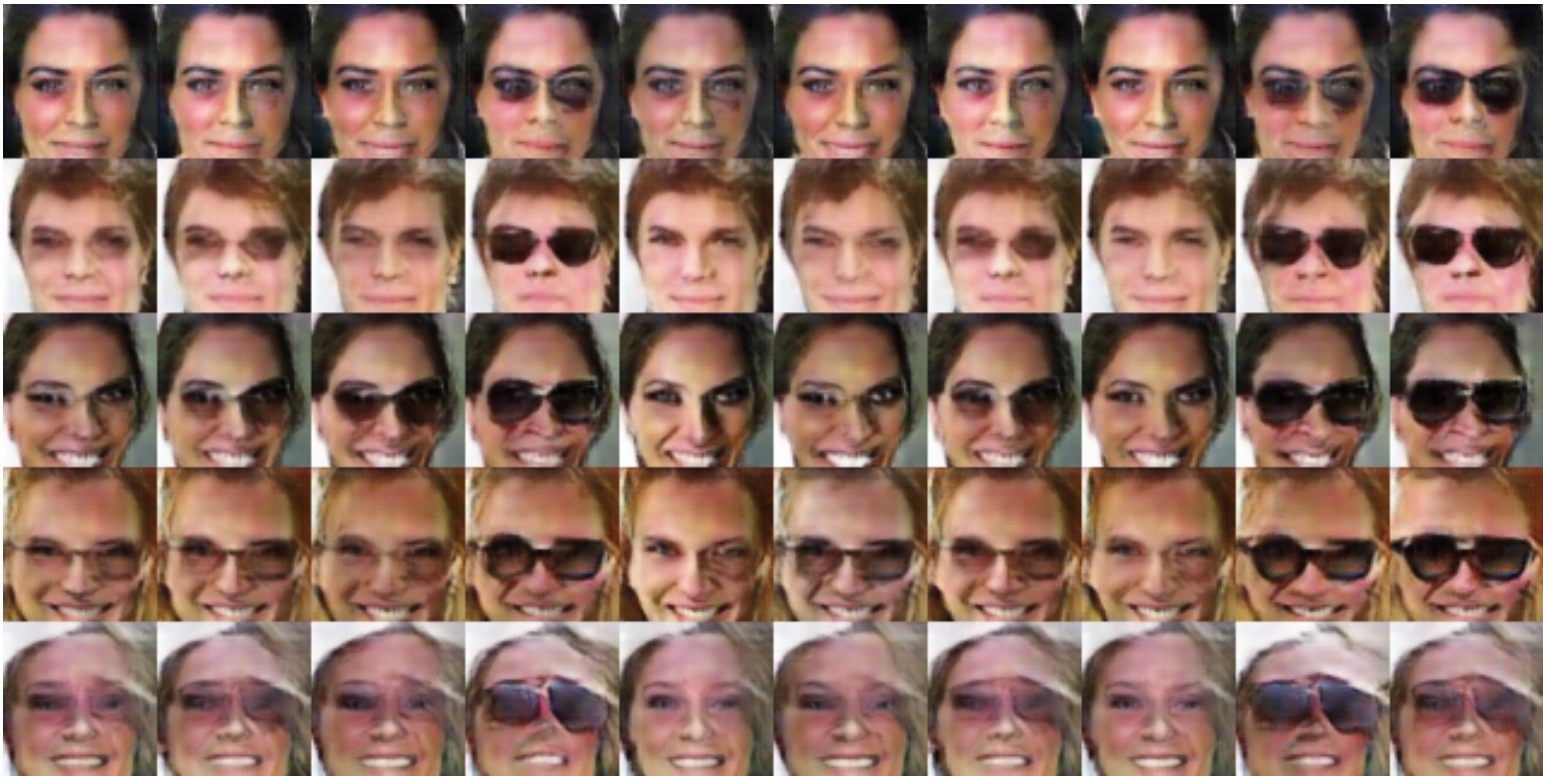
\includegraphics[width=5.0in]{infoGANglass.png}}
\caption{对抗生成网络生成图片的局限性}
\end{figure}

主要有以下几点原因:
.对抗生成网络的原理是拆解训练图片中的图像分布因子,将其储存在网络的参数之中,而随机噪声的输入,随着不断反卷积的操作,将输出的模式不断固化并且最终映射回原本的图像空间,其实是一个低维向高维投射的过程,但是因为投射的两维其实都是具有无限可能的,所以确实有完成这种也映射的可能,更何况人脸认为现实中存在的脸本身的范围就要比图像空间所能表示的范围要小得多。
但是基于目前CNN方法的对抗生成网络的原理是学习数据中的图像分布和梯度下降法的学习方法其实核心是针对于损失函数的优化,虽然在WGAN中对于对抗生成网络的损失函数又一次做出了优化,但依然不能够完美的和我们的任务相匹配,我们甚至不清楚自己想要的groundtruth是什么样的,所以损失函数的制定其实还不够出色,这也是为什么对抗生成网络的输出虽然显得很惊艳,但大多数时候还是会给人一种不真实感觉的原因。
所以在没有合格的损失函数之前,是不能够使用现有的对抗生成网络来进行神经网络的监督学习训练的,因为对抗生成网络生成的图片并不能真实的代表真实图片的分布。

但是在本论文的实验后期,我们想到了使用对抗生成网络来尝试迁移学习上的能力,其中使用了对抗生成网络在超分辨率上的应用。
\subsection{使用对抗生成网络提高人脸分辨率}
在发现对抗生成网络其实并不能直接从噪声生成具有一定训练意义的图片之后,我们并没有气馁。在参考了很多具有使用意义的对抗生成网络工作之后,决定从超像素的方向重新研究。超分辨率是通过硬件或软件的方法提高原有图像的分辨率的过程。在人脸超分辨率的之中,核心的思想就是在不改变人脸身份信息和属性信息的情况下,将人脸图像的更多细节还原出来。
\subsubsection{使用对抗生成网络生成高分辨率的图片}
在借鉴了了超分辨率的框架之后,设计了超分辨率神经网络框架是TRGAN\cite{TRGAN},
\begin{figure}[!ht]
\centering
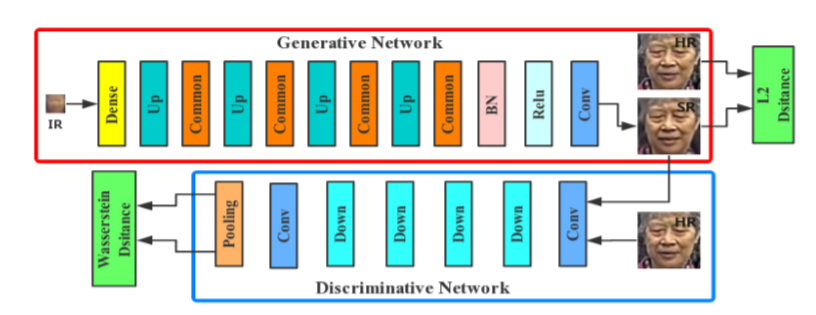
\includegraphics[width=6.0in]{TRGAN.png}
\caption{人脸超分辨率所使用的网络结构}
\end{figure}

具体来讲:
common模块:参考了resnet\cite{RESNET}的block模块,输入特征图分成两个分支,一个分支接BatchNorm之后接卷积层,再接一层batchnorm层和一层卷积层,最后该分支的block输出的特征图与另一个未经操作的分支使用元素对位相加(elementWise)。其目的是为了增加网络的深度,同时又能够为多层特征的融合提供不同的通道。

upSample模块:
在common模块的基础上,输入层的第一个分支连接到第一层卷积之后使用pixel shuffle\cite{ESPCN}的操作之后将图像尺寸变为原来的2倍。然后再接一层BatchNorm和卷积;
与此同时,第二层分支使用常规的双线性插值的方法扩大到两倍大小,使用1x1卷积连接之后将两个分支elementWise相加。
upsampling的操作相比common层的操作,可以让特征图变为原来的两倍大小,又增加了一定的特征融合。

downsample模块:
downsample的操作在common的基础上分别在两个分支的后面加入了stride为2的pooling层,可以保证输出特征图的大小为原来的一半。
\begin{figure}
\centering
\subfigure[Common模块]{
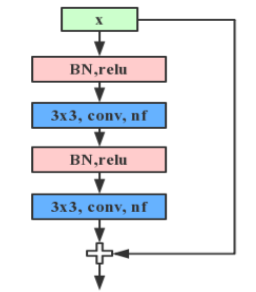
\includegraphics[width=1.50in]{a_common.png}
}
\subfigure[UpSample模块]{
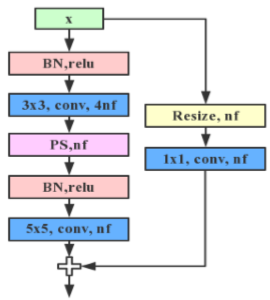
\includegraphics[width=1.50in]{b_up.png}
}
\subfigure[DownSample模块]{
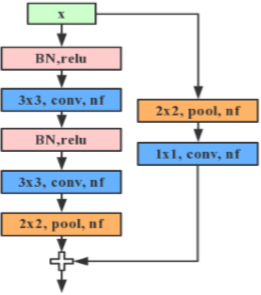
\includegraphics[width=1.50in]{c_down.png}
}
\caption{TRGAN中基于resnet的三种网络结构改进}
\end{figure}
使用该框架在celeA数据集上进行性训练,其中输入是8*8的低分辨率人脸,输出是64*64的高清人脸。优化的损失函数分别是输出的图片与原始高清图片的差值以及WGAN中的Wasseserstein Distance.
\begin{equation}{
W(P_r, P_g) = \frac{1}{K} \sup_{||f||_L \leq K} \mathbb{E}_{x \sim P_r} [f(x)] - \mathbb{E}_{x \sim P_g} [f(x)]
}
\end{equation}
具体的超分辨率实验结果:
\begin{figure}[!ht]
 \centering 
	\subfigure[缩小的16*16小图]{
	
\includegraphics[width=0.25in,height=0.25in]{lr_Aaron_Eckhart_0001.jpg}
	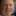
\includegraphics[width=0.25in,height=0.25in]{lr_Aaron_Guiel_0001.jpg}
	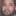
\includegraphics[width=0.25in,height=0.25in]{lr_Aaron_Patterson_0001.jpg}
	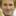
\includegraphics[width=0.25in,height=0.25in]{lr_Aaron_Peirsol_0001.jpg}
	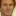
\includegraphics[width=0.25in,height=0.25in]{lr_Aaron_Peirsol_0002.jpg}
	}
	\subfigure[缩小的64*64原图]{
	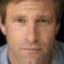
\includegraphics[width=1.0in,height=1.0in]{hr_Aaron_Eckhart_0001.jpg}
	
\includegraphics[width=1.0in,height=1.0in]{hr_Aaron_Guiel_0001.jpg}
	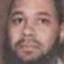
\includegraphics[width=1.0in,height=1.0in]{hr_Aaron_Patterson_0001.jpg}
	
\includegraphics[width=1.0in,height=1.0in]{hr_Aaron_Peirsol_0001.jpg}
	
\includegraphics[width=1.0in,height=1.0in]{hr_Aaron_Peirsol_0002.jpg}
	}
	\subfigure[超分辨率的64*64小图]{
	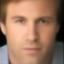
\includegraphics[width=1.0in,height=1.0in]{sr_Aaron_Eckhart_0001.jpg}
	
\includegraphics[width=1.0in,height=1.0in]{sr_Aaron_Guiel_0001.jpg}
	
\includegraphics[width=1.0in,height=1.0in]{sr_Aaron_Patterson_0001.jpg}
	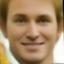
\includegraphics[width=1.0in,height=1.0in]{sr_Aaron_Peirsol_0001.jpg}
	
\includegraphics[width=1.0in,height=1.0in]{sr_Aaron_Peirsol_0002.jpg}
	}
	\caption{超分辨率使用lfw图片的效果示意图}
\end{figure}

可以看到对抗生成网络在超分辨率领域上取得了非常好的效果,可以在基本不改变人脸属性和身份信息的情况下,获取高清的图片。但是我们也发现一些有趣的现象:生成的图片虽然基本的轮廓不变,但是整体都相比原来更加白皙明亮了一些,整体给人的感觉都更加好看了一些。这其实是因为训练数据的图片都是celeA中的明星,其图片质量都比较出色,画风也带有一定的电影元素,似乎是把celeA的风格带到了lfw中,于是我有了一个大胆的想法。
\section{结合对抗生成超像素实现迁移学习}
\subsection{人脸属性的监督式学习困境}
首先引入一个经典的模式识别场景,泛化能力的问题:
在之前的工作种,经常可以发现一个经常出现的问题,使用MTL的人脸属性框架进行人脸属性识别的过程中,具同样40个属性标签的两个数据集lfwA和celeA,两个在各自数据集上训练之后的模型,在各自数据集上的准确率都很高,但是在对方的测试集效果都比较糟糕。

如何进行改善呢?我们针对于这种情况设计了这样的思路:
问题引出:对于相同的网络模型,使用相同的训练方法,在不同数据集中的训练之后,对自身数据集的测试集准确率要远远高于其他数据集的测试集。
问题分析:首先这不是一个过拟合问题,因为对于数据集中训练集和测试集的准确率较高,所以网络的训练没有问题。但是对于不同数据集的测试集准确率很低,所以推测问题的出现是因为数据的分布不同

尝试解决办法:首先我们先假定网络模型容量可以容纳两个数据的分布(数据的分布可能不满足线性加法,但是应该满足集合性合并不减的特性,所以假定两种数据的分布集合会比原来更大,所以对于网络容量的要求会更大),既然数据的分布不同,就应当减少数据分布对于模型训练带来的影响。

第一种方法就是将两个数据集合并训练,如果标签相同,那么可以简单的将两个数据集合并成一个数据集训练,也可以首先在一个数据集上份训练,再经过另一个数据集finetune,又或者采用上一章所提到的主干网路参数共享,不同数据集分别使用一个网络支线进行训练。都可以直观地学习到两个数据集之间的数据分布。往往就可以取得较好的效果,有效的提高在不同数据集上准确率的表现。

缺点:最致命的缺点就在于不同数据集的准确率提高,但是难以保证在自身的数据集上数据的准确性。即使采用较小的学习率谨慎的进行finetune,对于不同任务的训练过程也即将面临着大量的手动干预,还是处于一个监督学习的框架之中。

对此我们决定使用类似于迁移学习的方式来完成这个任务,并且结合对抗生成网络来完成我们的任务。
\subsection{人脸属性的迁移学习猜想}
迁移学习\cite{TRANSFER}是把一个领域(即源领域)的知识,迁移到另外一个领域(即目标领域),使得目标领域能够取得更好的学习效果。通常,源领域数据量充足,而目标领域数据量较小,迁移学习需要将在数据量充足的情况下学习到的知识,迁移到数据量小的新环境中。在图像领域,最主要完成迁移学习的方式就是将在源领域训练得到的模型作为特征提取器,然后在新的环境下使用诸如SVM、boosting等方式进行特征学习。或者固定模型的主要参数层,只重新训练后面针对于场景输出的特征提取类别。然后作为新环境的模型。

通常意义上的finetune,metric Learn ing也是迁移学习的分支。
而实际上迁移学习并没有明确的范围,其主要的目的是如何利用好已经学习到的知识,并将其应用到实际的应用场景之中。但实际场景虽然没有标注的数据,也是可以通过其他手段获取的知识,也就是说实际场景其实本身也是一种已经存在的知识,我们使用一些技巧将其已有的这是提取出来,并融合现有知识,完全有可能获得更加好的目标域识别效果。
\subsection{基于人脸超分辨率的人脸属性迁移学习实验}
在发现可以通过对抗生成网络将低分辨率人脸分辨率提高之后,我们设计了实验来针对上述问题进行研究。决定在lfwA的训练过程中混入超分辨率生成的LFWA人脸图像,目的也很明显,就是希望这些超分辨率的图片能够把celeA中的图像分布带到lfw中,从而提升使用lfwA数据训练的模型在在celeA数据上的性能。

实验中使用的网络是改进的alexnet主网络加上40个二分类的子网络模块。卷积层中的stride全部为1,保证网络特征图尺寸最后不会为消失。输入大小为64*64的人脸,通过上一章中提到的人脸矫正作为预处理的方式。使用人脸识别的与训练模型作为预训练基础。数据混合策略是按照将超像素图片和lfwA的原始图片按照1:1的比例作为训练数据。

实验结果如下:
\begin{table}[!h]
  \centering
   \caption{在CELEA数据集}
   \begin{tabular}{c|c|c}
     \toprule
     数据集训练 &数据集测试 &40属性平均准确率\\
     \midrule
      LFWA   &  CeleA &  66.2 \\
	  CeleA  &  CeleA &  89.1 \\
	  LFW-hr &  CeleA &  76.2 \\
      LFWA   &  LFWA  &  83.4 \\
	  CeleA  &  LFWA  &  70.7 \\
	  LFW-hr &  LFWA  &  83.3 \\
     \bottomrule
   \end{tabular}
\end{table}
\section{实验结果分析与结论}
从训练的结果来看可以看出,使用celeA训练数据的模型,在celeA测试集中取得了89.1\%的准确率,但是在lfwA上的准确率就降低了和蒂诺。只有70.7\%。类似的使用lfwA数据进行训练,也具有同样的现象。这符合人脸属性种监督学习的困境。
再加入了人脸超分辨率像素的进行训练之后,情况有了改善,不仅使用超分辨率像素训练的模型在原本的lfwA数据集上具有良好的效果,只是下降了0.1个百分点,在celeA数据集上也提升10个百分点。这说明基于超分辨率的像素来完成人脸属性识别是可行的。通过改变训练数据的情况下,对数据的预处理过程添加了一定其他环境噪声分布,这和传统通过数据增强的方式完成的数据噪声加入是有很大不同的。原始的数据增强例如平移、旋转、色彩通道等变换等都还是对于现有数据分布从离散化的输入到连续化扩充,是可以充分的利用输入数据的分布资源。但超分辨的图像变换形式其实可以更深层次的改变图像的状态而最大限度保留图像的标注信息不发生改变。这样是最直接的增加数据分布的方式。尤其是在本实验中lfwA中的图片数量较少,数据的分布也更加偏僻且具有离散化,和celeA也有很大的差距,简单的数据增强其实并不能完全解决这个问题。所以使用超分辨率的方式进行扩充训练可以取得更好的效果。

但是不得不承认,虽然本文中没有常熟将celeA和lfwA数据进行混合训练的方式,但是无疑这样的方式其实最直接提升在不同数据场景下识别效果的方式,而且流程更加简单,使用训练数据并行的训练方式其实是可以取得优异的效果的。然而基于超分辨率的迁移学习的优势其实体现在对于未知数据场景的学习能力。在现有数据中进行模型的学习,然后针对于不同的数据场景,使用超分辨率的模型对于场景图片进行学习和复现,这样可以轻松从有标注的数据的低分辨率版本获得有标注数据在对应场景的移植高分辨率版。再将移植的高分辨率的图像通过正常训练的图片。

\section{本章小结}
在本章中首先对于对抗生成网络的相关技术做了介绍,然后研究了对抗生成网络现实中比较常见的应用包括使用对抗生成网络生成真实图像和使用对抗生成网络提高图片的分辨率。在探究和实验的过程之中,我们完成了相关的图片生成任务,g对抗生成网络也体现出了非常令人眼前一亮的伪造图片能力。但针对于人脸属性任务对于图片的要求,生成图片依然很难满足相关的真实程度和标签要求。

但是使用超分辨率对于低分辨率人脸的修复和生成体现了良好的效果。于是结合迁移学习的方式,我们对于人脸属性识别在不同场景的识别效果做了探究性实验。
总结来说,迁移学习是监督学习之后最具有研究方向的领域,我们对此进行探究,并发现在我们固定的实验方法和celeA与lfwA 40种属性分类的场景下,使用基于超分辨率的学习方法确实可以有一定的效果提升。
\chapter{总结与展望}
\section{全文总结}
通观全文,与其说实在研究如何提高人脸属性的识别准确率,倒不如说是在各种偏离基础算法使用场景的情况下,解决一个又一个出现的问题,包括
为了能够提高训练速度,在训练中的不同框架,尝试探究多机多卡。
为了在实际测试中,具有较高的反馈和实用价值,在基础的神经网络操作中,对于基本算法的加速和改进。
为了适应针对数据集训练和评测的这种模式,设计针对于多种属性标签,多种数据集的网络架构。
为了对于不同的场景数据分布存在偏差的问题,针对于背景的变化,使用gan网络对于人脸图片进行了所谓的场景人脸重构。
在这个过程中,不仅对于模式识别的基本算法有所掌握,同样也印证着发现问题,分析问题和解决问题的思路。
从学术研究的贡献来看,其实并没有提出提别的足够具有改变行业性的算法,更像是对于现有算法更加深入和具体化的改进。
从整个研究任务的完成上,主要的思考点和实现的标准有两方面:
一方面从底层实现上探究在目前计算机水准上,热衷于探究对于算法的实现能够具有怎样的加速方法,让算法的实现和使用变得快速化。
另一方面在常规的网络构建上思考如何能够构建更加具有端到端的特性,让机器学习的相关问题分析和解决流程变得更加简洁化。
仅此而已。

总体自我评价来看,还需要更多

\section{未来展望}
本文所介绍的人脸属性识别属于图像识别种基于监督学习的分支,同时也是非常具有代表性的任务之一,类似的人物包括物体识别中的物体性质识别,如经典的鱼种类识别等。
所以人脸属性识别的进展需要依托于整个图像识别的基础技术进展和图像数据库的建设。而图像识别领域基础技术的进展其实更加依托于更加基础计算机科学的进步与发展,细节小到晶体管的制造工艺,计算机内存和缓存的读取速度,处理器的主频提升,布局大到整个体系结构的变革,冯诺依曼体系的变革,量子计算机的进化等,都会对于模式识别算法有着较为深远的影响。

除了对于底层科学的依赖,现实生活中的应用落地也同样具有重大意义,比如慢慢成熟的人脸识别,自动驾驶等新兴技术行业,无一不是有基础的模式识别技术发展而来,但是却无一不在现实的产业结构中引发巨大热潮,让实验室的算法走出实验室出现在人们的现实生活种,可以极大激励人们对于人工智能的探索的热情和改变人类生活状态的前行动力。并且在实际生活中慢慢探索图像识别的规律,加速人工智能领域的快速发展。



 

%% 附录部分

%% 如果只有一个附录, 使用appendix*环境
%% \begin{appendix*}
%%   % 自动抽取生成缩略语表作为附录A
%%   % \tableofacronyms
%% \end{appendix*}

\ifx\usechapbib\undefined
\bibliographystyle{buptgraduatethesis}
\bibliography{bare_thesis}
\fi

\backmatter
%% 致谢
\ifx\ispeerreview\undefined
%%
%% This is file `example/ackgmt.tex',
%% generated with the docstrip utility.
%%
%% The original source files were:
%%
%% install/buptgraduatethesis.dtx  (with options: `ackgmt')
%% 
%% This file is a part of the example of BUPTGraduateThesis.
%% 

\begin{acknowledgement}
  %% 感谢所有你应该感谢的人
  感谢自己,感谢所有人.
\end{acknowledgement}

\fi

%% 在读期间论文发表情况
%%
%% This is file `example/pubs.tex',
%% generated with the docstrip utility.
%%
%% The original source files were:
%%
%% install/buptgraduatethesis.dtx  (with options: `pubs')
%% 
%% This file is a part of the example of BUPTGraduateThesis.
%% 

%% 发表论文列表

%% 攻读学位期间发表论文列表用 tableofpublications 环境产生。需要
%% 在 bare_thesis.tex 的导言区用 \newcite{<name>}{<caption>} 声明不同类
%% 型的论文,具体见导言区说明。
%% 根据各类论文发表数量设置\setbiblabelwidth{<num>},用于控制发表论文序号的对齐位置。
%% 例如:发表conf类论文数量为个位数,则<num>=1;发表jrnl类论文数量为两位数,则<num>=10;



\newpage
\end{document}
